\section{Privacy degli utenti}
Il desiderio degli utenti è quello di non dover sempre dichiarare la loro identità quando eseguono qualcosa nel cloud. Per questo entrano in gioco:
\begin{itemize}
    \item tecniche di comunicazione anonima
    \item privacy basata sulla locazione
    \item controllo di accesso su attributi
    \item preferenze di privacy che l'utente ha quando interagisce col sistema
\end{itemize}
\subsubsection{User empowerment}
Gli utenti potrebbero voler specificare le policy che regolano le informazioni divulgate quando usano servizi esterni per condividere le loro risorse (Facebook) o quando rilasciano informazioni in interazioni digitali (carte di credito quando accedo a un determinato servizio). \\
Dobbiamo quindi proteggere due aspetti:
\begin{itemize}
    \item rilascio diretto, regola da chi, quando e con che scopo un utente è d'accordo a rilasciare delle informazioni
    \item uso secondario dei dati, regola l'uso e la condivisione dei dati che erano usati per uno scopo primario
\end{itemize}

\subsubsection{Rilascio diretto}
La comunità di ricerca è stata molto attiva in questo ambito è ha prodotto diversi approcci che regolano le interazioni tra le parti basate sulla definizione di meccanismo \textbf{attribute-based access control}:
\begin{itemize}
    \item cosa un utente può fare in base agli attributi che presentano nel loro certificato
    \item il controllo di accesso non risponde più sì/no, ma risponde con una lista di requisiti che il richiedente del servizio deve soddisfare per ottenere l'accesso
\end{itemize}
Inoltre non dobbiamo pensare a garantire la sicurezza solo al server ma anche il client vuole le sue garanzie, magari introducendo qualche forma di negoziazione.\\
Vediamo tre modalità di Interactive Access Control:
Controllo di accesso senza condizioni dal client (troppo semplice):
\begin{center}
    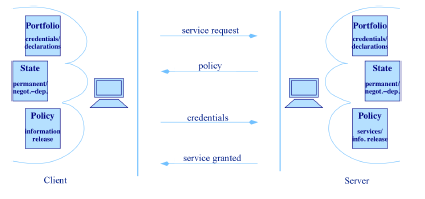
\includegraphics[scale=0.6]{img/iac1.png}
\end{center}
Controllo di accesso senza condizioni dal client, ma con negoziazione (troppo complicato):
\begin{center}
    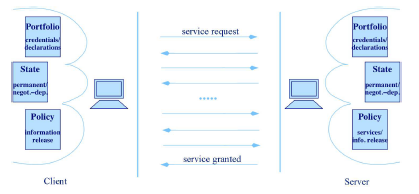
\includegraphics[scale=0.6]{img/iac2.png}
\end{center}
Controllo di accesso senza condizioni dal client, con two step interaction:
\begin{center}
    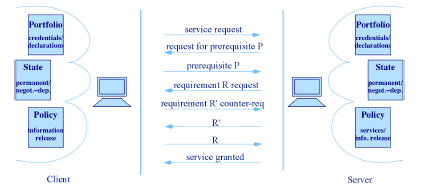
\includegraphics[scale=0.6]{img/iac3.png}
\end{center}
Esistono tecnologie che supportano ABAC e sono:
\begin{itemize}
    \item U-Prove/Idemix: forniscono un avanzato sistema di gestione delle credenziali
    \item XACML: standard per interoperazioni di controllo di accesso
\end{itemize}

\subsubsection{User privacy preferences}
Le specifiche di controllo di accesso non sempre riescono a coprire anche il problema dal lato dell'user, infatti non permettono all'utente di esprimere la preferenza di rilasciare alcune informazioni rispetto a delle altre.
\begin{itemize}
    \item \textbf{Context-based}: rilascio la mia carta di credito solo quando devo effettivamente pagare
    \item \textbf{Forbiden disclosures}: non voglio rilasciare allo stesso server il mio vero nome e il mio nickname
    \item \textbf{Sensitive associations}: il mio ZIP code e la data di nascita sono più sensibili quando sono insieme
    \item \textbf{Limited disclosure}: ti dico se sono maggiorenne ma non ti dico la mia età precisa
    \item \textbf{History-based}: ti do la provincia di residenza invece del mio telefono se possiedi già il mio indirizzo
    \item \textbf{Proof-based}: posso dimostrare qualcosa senza rilasciare il documento, ad esempio dimostro di essere italiano senza rilasciarti il passaporto
    \item \textbf{Non-linkability}: preferisco rilasciare dei pezzi di informazioni che se messe insieme mi rendono il meno identificabile possibile
\end{itemize}

Successivamente approfondiremo qualche approccio, tra cui:
\begin{itemize}
    \item Cost-sensitive trust negotiation
    \item Point-based trust management model
    \item Logic-based minimal credential disclosure
    \item Privacy preferences in credential-based interactions
\end{itemize}

\subsection{Cost-sensitive Trust Negotiation}
Due parti (client e server) interagiscono tra di loro stabilendo fiducia reciproca scambiandosi credenziali (trust negotiation protocol). \\ Credenziali e policies sono associate a un costo, dove più le credenziali o le policies sono sensibili, più il costo è alto.\\
L'obiettivo è quello di minimizzare il costo totale di sensibilità di credenziali e policies durante una trust negotiation.
\begin{center}
    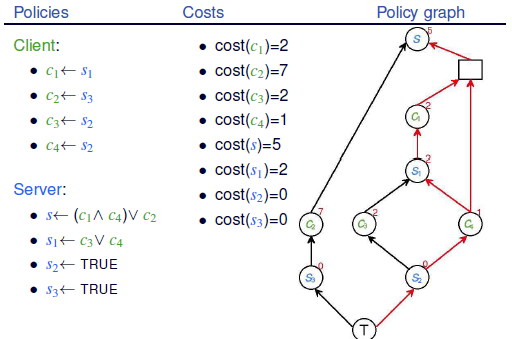
\includegraphics[scale=0.6]{img/csens.png}
\end{center}
In questo esempio il client ha quattro credenziali: c1, c2, c3 e c4.\\
Il server ha tre credenziali s1, s2, s3 e il servizio s a cui dà accesso.\\
Le politiche che sono implementate sono del tipo "se mi dai questo, ti rilascio questo". Quindi, lato server: s2 e s3 vengono sempre rilasciati, s1 viene rilasciato solo se mi presenti c3 o c4 e s viene rilasciato se mi presenti c1 e c4 oppure in alternativa c2. Il client invece dice: rilascio c1 se mi dai s2, c2 se mi dai s3 e c3 e c4 se mi rilasci s2. \\
Il percorso scelto alla fine è evidenziato in rosso e viene scelto proprio quello perchè è minima la somma dei costi.\\
Questo metodo fornisce un meccanismo per regolare il rilascio delle credenziali in accordo con la loro sensibilità e pone il suo focus sulla negoziazione più che sul controllo del client. Inoltre minimizzare il costo totale ha applicazioni limitate. Una combinazione lineare di costi potrebbe non essere sempre desiderata.

\subsection{Point-based Trust Management Model}
Chi possiede il servizio dà un certo numero di punti per ogni credenziale. Quindi per accedere ad un certo servizio servono un tot di credenziali (questa soglia viene mantenuta privata). Anche il client valuta le sue credenziali con un punteggio privato che indica la sensibilità dell'informazione. L'obiettivo diventa quindi quello di raggiungere il punteggio del server dando meno informazioni sensibili possibili.\\
\begin{center}
    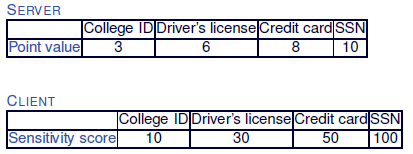
\includegraphics[scale=0.6]{img/pointbased.png}
\end{center}
Supponiamo che bisogna fornire almeno 10 punti per accedere a una risorsa.\\
Le opzioni che ha il client sono:
\begin{itemize}
    \item SSN [10 punti, 100 di sensibilità]
    \item College ID, Credit Card [11 punti, 60 di sensibilità]
    \item Driver's license, Credit Card [14 punti, 80 di sensibilità]
\end{itemize}
L'opzione numero due è quindi la migliore.\\
Il problema è che bisogna continuare a fornire dati fino a che non abbiamo raggiunto la soglia (Credential Selection Problem).\\
La soluzione è convertire il problema in un knapsack problem e risolverlo con un approccio di programmazione dinamica. Più esattamente viene utilizzato un protocollo di programmazione dinamica sicuro e a due parti:
\begin{itemize}
    \item il server e il client calcolano insieme la somma ottima dei punti senza rivelare i loro punteggi
    \item il protocollo usa hosomorphic encription, ossia l'operazione viene fatta sui dati criptati (equivale a decriptare, fare l'operazione e criptare)
\end{itemize}

Il modello point-based ha quindi queste caratteristiche:
\begin{itemize}
    \item client e server devono mettersi d'accordo sulle credenziali e avere quindi un'ontologia comune
    \item ogni credenziale è considerata come un'unità
    \item mette il focus sulla negoziazione più che sul controllo del client
\end{itemize}

\subsection{Logic-based Minimal Credential Disclosure}
Le parti sono coinvolte in una negoziazione fidata dove il rilascio delle credenziali è regolato da delle policies. Ogni credenziale è un singolo attributo. Le diverse policies formano un grafo.
\begin{center}
    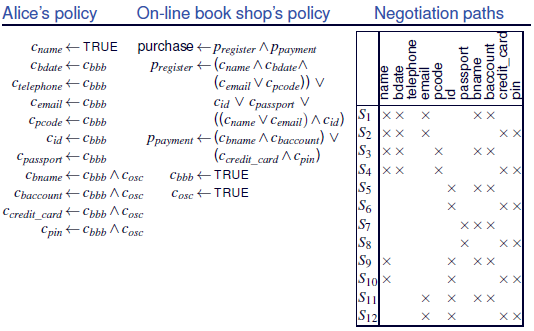
\includegraphics[scale=0.6]{img/logic.png}
\end{center}
La tabella di negoziazione può essere vista come una tabella binaria dove 0 indica il non rilascio, 1 indica il rilascio.\\
\begin{center}
    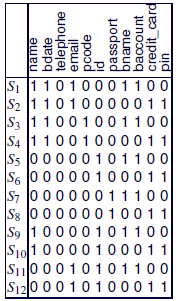
\includegraphics[scale=0.6]{img/logbin.png}
\end{center}
La preferenza di default è ovviamente quella di non rilasciare una credenziale piuttosto che rilasciarla:
\[ \Longrightarrow 0 \succ_i 1 \]
con i che rappresenta la i-esima credenziale. I set di rilascio sono comparati attraverso la \textbf{Pareto composition} (\(\succ_p\)), dove:\\
\(s_i\) domina \(s_j\) se \(s_i\) mostra un valore migliore o uguale a \(s_j\) rispettando la preferenza di credenziali ed è strettamente migliore con il rispetto di almeno una credenziale.\\
Ad esempio: presi \(s_5 : [0, 0, 0, 0, 0, 1, 0, 1, 1, 0, 0]\) e \(s_9 : [1, 0, 0, 0, 0, 1, 0, 1, 1, 0, 0]\) 
notiamo come \(s_5[1] \succ_1 s_9[1]\) mentre gli altri valori sono uguali. Questo vuol dire che \(s_5\) domina \(s_9\) e più precisamente \(s_5 \succ_p s_9\).\\
Introdurre delle gerarchie ci permette di poter definire la preferenza di rilascio di una credenziale rispetto ad un'altra e introduce anche la transitività.\\
Le caratteristiche di questo modello sono:
\begin{itemize}
    \item utenti coinvolti nella scelta del set da rilasciare
    \item si basa sugli attributi e non sulle credenziali
    \item non sempre è facile esprimere le preferenze degli utenti tra gruppi di attributi
    \item la possessione di credenziali sensibili non è considerata
    \item rilasci vietati non sono supportati
\end{itemize}


\subsection{Privacy Preferences in Credential-based Interactions}
L'obiettivo è quello di permettere all'utente di regolare effettivamente il rilascio delle sue proprietà e delle sue credenziali:
\begin{itemize}
    \item identificare i requisiti e i concetti che devono essere catturati
    \item organizzare le proprietà dell'utente e le credenziali nel suo portfolio
    \item abilitare l'utente ad esprimere quanto ritiene sensibili il rilascio di certe properietà presenti nel portfolio
    \item fornire possibili approcci tecnici per supportare le preferenze dell'utente
    \item fornire una base per investigare approcci user friendly per regolare il rilascio delle proprietà
\end{itemize}
\subsubsection{Modellare il Portfolio}
Abbiamo citato in questi punti il portfolio dell'utente, ma esattamente cosa vuol dire modellare il suo portfolio?
\begin{itemize}
    \item Credenziali: certificati verificati e firmati da qualcuno che certifica le proprietà. Una credenziale di solito possiede un type, un identifier e un issuer (chi l'ha rilasciata)
    \item Dichiarazioni: una credenziale autofirmata
\end{itemize}
Il portfolio ha diversi tipi di proprietà:
\begin{itemize}
    \item indipendenti: il valore dipende solo dal proprietario delle credenziali
    \item dipendenti: il valore dipende dalla credenziale certificante (il numero di carta di credito varia in base alla carta di credito)
\end{itemize}
Allo stesso modo, il portfolio ha diversi tipi di credenziali:
\begin{itemize}
    \item atomiche: quando rilascio un certificato lo rilascio tutto (ad esempio la carta d'identità, perchè con lei rilascio il nome, il cognome ecc ecc)
    \item non atomiche: posso selezionare cosa rilasciare (ad esempio la patente, dove non sono obbligato a dare tutte le informazioni)
\end{itemize}
Un rilascio è un subset del portfolio dell'utente che soddisfa:
\begin{itemize}
    \item certificabilità: ogni proprietà è certificata da una credenziale
    \item atomicità: se viene rilasciata una proprietà di una credenziale atomica, tutte le sue proprietà vengono rilasciate
\end{itemize}
Parti diverse di un portfolio hanno diversi livelli di sensibilità (l'utente infatti potrebbe preferire rilasciare una proprietà x piuttosto che una proprietà y). Per poter effettuare questa diversificazione introduciamo delle \textbf{etichette di sensibilità} tra cui vale l'ordine parziale (ossia non abbiamo maggiore o minore stretto, ma maggiore e minore uguale) e sulle quali è definito un operatore di composizione \(\oplus\) (la composizione di due etichette di sensibilità è un'altra etichetta di sensibilità)

\subsubsection{Sensibilità di proprietà e credenziali}
\(\lambda(A)\): sensibilità della proprietà A presa individualmente.\\
\(\lambda(c)\): sensibilità dell'esistenza della credenziale c

\subsubsection{Sensibilità delle associazioni}
\(\lambda(A)\): sensibilità dell'associazione \(A = \{A_i,...,A_j,c_k,...,c_n\}\), il cui rilascio congiunto porta:
\begin{itemize}
    \item più informazioni che il rilascio di ogni elemento in A \textbf{(sensitive view)}
    \item meno informazioni del rilascio di ogni elemento in A \textbf{(dependency)}
\end{itemize}

\subsubsection{Vincoli di rilascio}
Dato il set \(A = \{A_i,...,A_j,c_k,...,c_n\}\) di elementi il cui rilascio deve essere controllato abbiamo:
\begin{itemize}
    \item \textbf{forbidden view}: il rilascio di A è proibito
    \item \textbf{disclosure limitation}: almeno n elementi in A possono essere rilasciati
\end{itemize}
Un rilascio è valido se non viene violato nessun vincolo

\subsubsection{Sensibilità del rilascio}
La sensibilità \(\lambda(D)\) di un rilascio D è la somma delle etichette di sensibilità che sto rilasciando, considerando proprietà, credenziali e associazioni. Ad esempio:
\begin{center}
    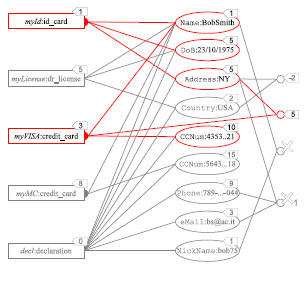
\includegraphics[scale=0.6]{img/discsens.png}
\end{center}
in questo caso abbiamo che le proprietà valgono 1+5+5+10, le credenziali 3+1 e le associazioni 5. In totale\(\lambda(D)\) = 30

\subsubsection{Server Request}
La richiesta R è una semplice disgiunzione (OR) di richieste semplici, dove una richiesta semplice r è data da una congiunzione (AND) di termini. \\
Ad esempio:\\
R = \( r_1 \lor r_2\) \\
\( r_1 = id.\{Name, Address\}\) \\
\( r_2 = cc.\{Name, CCNum\}\) \\
Data la richiesta R come fa il client a decidere quali credenziali rilasciare? Devo trovare un insieme che soddisfi la richiesta del server e che abbia la minore sensibilità possibile.

\subsubsection{Problema del Rilascio Minimo}
Un rilascio D:
\begin{itemize}
    \item soddisfa R, ossia soddisfa almeno una delle r in R
    \item soddisfa r se per ogni credenziale richiesta il client presenta una credenziale del tipo richiesto e che certifichi quelle proprietà
    \item è minima se non esiste un rilascio D' migliore
\end{itemize}
Calcolare il problema del minimo rilascio è NP-hard e abbiamo due modalità per risolverlo:
\begin{itemize}
    \item sfruttare la rappresentazione del grafo e vedere se esistono euristiche in grado di risolvere il problema
    \item tradurlo in un problema di soddisfacibilità booleana così da usare SAT solver: in pratica ho delle variabili booleane e una  formula da soddisfare. Devo trovare quindi un assegnamento alle variabili che mi renda la formula vera. Max-SAT è massimizzare il numero delle variabili soddisfatte, ma a noi serve il contrario, dato che dobbiamo minimizzare (ci basta tradurre Max-Sat in forma negativa)
\end{itemize}

\subsubsection{Server side}
XACML è uno standard utilizzato per interoperabilità di politiche di controllo di accesso. Questo però ha diversi limiti:
\begin{itemize}
    \item non fornisce la specifica della proprietà che deve essere certificata dal certificato
    \item non supporta le astrazione
    \item non supporta la politica del dialogo (per comunicare all'utente le policy)
    \item non supporta condizioni ricorsive (per esprimere policy basate su catene o su delegazioni)
\end{itemize}